\documentclass[spanish]{assignment}
\usepackage{url}
\usepackage{amsmath}
\usepackage{pdflscape}

% Title page
\title{Búsqueda y minería de información.}
\subtitle{Práctica 2 - Implementación de un motor de búsqueda}
\author{Guillermo Ruiz Álvarez\\ Enrique Cabrerizo Fernández}
\date{\today}
\university{Universidad Autónoma de Madrid}

\begin{document}
	\makepre
	\section{Ejercicio 1: Creación de Índices.}
	En este apartado se expondrán las decisiones tomadas para tratar de construir un índice en disco
	que sea capaz de indexar la colección de 100.000 documentos en un tiempo y con un consumo de RAM aceptables.
	
	\subsection{Algoritmo empleado.}
	Para la creación del índice se han tenido en cuenta diversas implementaciones analizadas por la universidad de Stanford, concretamente las opciones Blocked sort-based indexing (BSBI \footnote{BSBI:\url{http://nlp.stanford.edu/IR-book/html/htmledition/blocked-sort-based-indexing-1.html\#4947}})
	y Single-pass in-memory indexing (SPIMI\footnote{SPIMI:\url{http://nlp.stanford.edu/IR-book/html/htmledition/single-pass-in-memory-indexing-1.html\#5079}}).
	Finalmente se decidió adoptar el método SPIMI por ser más eficiente, $O(T)$ frente a $O(Tlog(T))$, donde T es el número total de tokens a procesar y por no necesitar una estructura para asociar términos a ids únicos.
	\\
	En la figura \ref{fig:spimi_pseudo} se puede ver el pseudo-c\'odigo b\'asico del algoritmo:
	\begin{figure}[h]
		\centering
		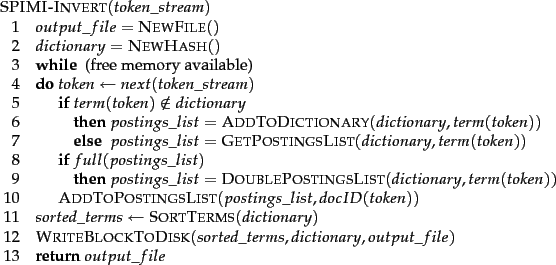
\includegraphics[width=0.8\textwidth]{SPIMI.png}
		\caption{Pseudo-c\'odigo SPIMI}
		\label{fig:spimi_pseudo}
	\end{figure}
	
	Nuestra implementación realiza una pequeña variaci\'on de este algoritmo.
	Cuando se quiere construir un \'indice, se ejecuta el m\'etodo \textit{build} de la clase \textit{BasicIndex} con los par\'ametros apropiados. Dicha clase parsea cada documento a indexar y finalmente ejecuta el método \textit{add}, de la clase \textit{IndexWriter}. Éste método es el que ejecuta el pseudocódigo descrito arriba con una salvedad: solamente se comprueba si se ha excedido el tamaño de bloque al terminar de añadir todo el documento, es decir, un documento nunca se guardará en dos bloques distintos. Esto impide que un \textit{posting} de un término sea escrito a disco cuando aún es posible que dicho t\'ermino vuelva a aparecer en el documento, lo que implicaría crear un nuevo posting para el mismo término y mismo documento. Esto más adelante obligaría en la fase de \textit{merge} a fusionar \textit{postings}, además de las propias listas de \textit{postings}.
	
	Teniendo en cuenta que los archivos a indexar ocupan menos de 100kB (antes de parsear HTML) y que nuestros bloques por defecto (archivos escritos en disco), son de 10 MB, se ha considerado aceptable que el tamaño de bloque sea orientativo, pudiendo oscilar hasta aproximadamente los 10.10 MB a cambio de ahorrar tiempo en la fase de \textit{merge}. De esta forma, solamente tendremos que realizar fusión de listas de \textit{postings}, algo trivial con las estructuras de datos que utilizamos, descritas en la sección \ref{est_datos}.
	
	Al terminar de añadir documentos al índice se fusionan todos los índices parciales creados en cada bloque hasta obtener un único índice. Para ello se han usado hilos que hacen \textit{merge} de los bloques 2 a 2, realizando un total de $\lceil log_2(k) \rceil$ \textit{merges} en total, siendo k el número de bloques generados.
	
	\subsection{Estructuras de datos.}\label{est_datos}
	\subsubsection{Creación del índice.}
	Durante la creación del índice mantenemos las siguientes estructuras de datos:
	\begin{itemize}
		\item Diccionario de bloque: Tabla hash con claves ordenadas (\textit{TreeMap}), en la que se guardan los términos como clave y sus listas de \textit{postings} como valor.
		\item Diccionario de Documentos: Tabla hash con asignaciones entre el nombre del documento (valor) a indexar y un id numérico único asignado al agregarlo al índice (clave). Esto nos permitirá guardar en las listas de \textit{postings} los ids numéricos y no los nombres de documentos ahorrando espacio. La tabla nos permitirá recuperar posteriormente el nombre del documento en las búsquedas.
	\end{itemize}
	\subsubsection{Merge.}
	Durante el último \textit{merge} que realiza el algoritmo, se guarda en una tabla hash adicional la información de la posición de cada término (\textit{offset}) dentro del índice para que la búsqueda posterior sea más eficiente. 
	De forma que para buscar un término, consultaremos en la tabla hash su \textit{offset} dentro del archivo en O(1) y accederemos directamente a esa posición para leer su lista de \textit{postings}.\\
	
	Como esto podría resultar demasiado costoso en RAM si el índice contuviera demasiados términos, se ha decidido implementar una versión que permite dividir el diccionario en bloques, cada uno de los cuales contiene \textit{TERM\_MAP\_SIZE} (ver \textit{IndexWriter}) términos, de forma que solamente el primer término de cada bloque se guarda en la tabla hash. De esta forma, para encontrar un término en el índice, consultamos el offset del mayor término menor que él (orden alfabético) en la tabla, y haremos busqueda lineal desde ahí. Por defecto se ha dado valor 100 al tamaño de bloque, por lo que si un término no es encontrado después de leer 100 términos, es que no se encuentra en el índice.\\
	
	Adicionalmente, se aprovecha la lectura de cada término en el momento del volcado al archivo de índice definitivo para calcular los módulos de los documentos (implementación orientada a términos), con lo que se guarda una estructura adicional (array) de módulos para cada documento de la colección.
	
	\subsection{Índice en disco.}
	Él índice en disco se encuentra en el archivo \textit{index} y consta de una sucesión de cadenas con el siguiente formato\footnote{Los corchetes no forman parte del archivo, se han puesto para añadir claridad}:
	\begin{align*}
	T\_S_T\{D_1N_1P_{D_11}P_{D_12}\cdots P_{D_1N_1}\}\cdots \{D_mN_mP_{D_m1}\cdots P_{D_mN_m}\}
	\end{align*}
	Donde cada letra representa lo siguiente:
	\begin{itemize}
		\item$T$: Término literal que se está leyendo, siempre va seguido de un espacio que indica el final del término, de forma que nuestro índice no acepta términos formados por varias palabras separadas por espacio.
		\item$S_T$: Tamaño en bytes de toda la lista de postings en disco del término $T$.
		\item$D_x$: Id del documento al cual pertenecen los postings que se leerán a continuación.
		\item$N_x$: Frecuencia del término en el documento $D_x$.
		\item$P_{D_xy}$: Valor de posición $y$ del término $T$ en el documento $D_x$.
	\end{itemize}
	
	Con esta estructura para cada término en los archivos el \textit{merge} cuando encontramos el mismo $T$ presente en dos bloques distintos es muy simple; simplemente se suman las $S_T$ y se concatenan los bytes posteriores, poniendo primero la cadena correspondiente al menor bloque (el que fue creado antes) para conservar el orden de los postings.
	
	Las tablas hash de ids de documentos y diccionario de términos con offsets, se guardan en disco en los archivos \textit{docids} y \textit{termsoffset}. El array de módulos de documentos se guarda en el archivo \textit{modules}
	Para crear estos archivos se ha hecho uso del método \textit{writeObject} de la clase \textit{ObjectOutputStream}, ya que permite recuperar los objetos fácilmente desde archivo mediante el método \textit{readObject}.
	
	\subsection{Parsing}
	
	La diferencia principal entre las tres clases de índice pedidas para este ejercicio se encuentra esencialmente en el \textit{parser} que utilizan. Tanto el índice de \textit{Stopwords} como el índice que realiza \textit{Stemming} realizan exactamente el mismo indexado que el índice básico, con la diferencia de que el contenido que añaden para cada archivo ha sido previamente \textit{parseado} de forma distinta. Por lo tanto, las tres clases de índice pedidas para este ejercicio, \textit{BasicIndex}, \textit{StopwordIndex} y \textit{StemIndex} se diferencian únicamente los argumentos con los que ejecutan la función \textit{build} desde el método \textit{main}.\\
	
	A continuación vemos qué hace cada \textit{parser}:
	\begin{itemize}
	\item Parser Básico (\textit{BasicParser}): Además de eliminar las etiquetas HTML, elimina todos los símbolos que no sean caracteres [a-zA-Z] y posteriormente transforma todo el texto a lower case.
	\item Parser de \textit{Stopwords} (\textit{StopwordParser}): Realiza el filtrado del parser básico y a continuación elimina los \textit{stopwords} y las palabras de longitud $\leq 2$.
	\item Parser de \textit{Stemming} (\textit{StemParser}): Realiza el filtrado de \textit{StopwordParser} y posteriormente utiliza el \textit{snowball stemmer} con diccionario inglés realizando dos pasadas sobre cada término.
	\end{itemize}
	
	\subsection{Algunos resultados}
	En la figura \ref{profilaxis} podemos ver la gráfica extraída con el \textit{profiler} de \textit{NetBeans} para la ejecución de la clase \textit{IndexBuilder} construyendo los tres índices sobre la colección de 100.000 documentos.\\
	
	Con \textit{output} auxiliar del programa se ha medido el tiempo de creación de cada índice, siendo éste aproximadamente de 27, 31 y 30 minutos para \textit{BasicIndex}, \textit{StopwordIndex} y \textit{StemIndex} respectivamente.\\
	
	Como se puede comprobar en la gráfica, el procesamiento de documentos es más largo en los índices con filtrado de \textit{stopwords} y \textit{stemming}, pero la fase de \textit{merge} se acorta, debido a la eliminación de más términos a consecuencia del filtrado.\\
	
	El consumo de RAM se mantiene en valores razonables, alcanzando picos máximos de 900 MB durante las fases de procesamiento de documentos en los índices \textit{StopwordIndex} y \textit{StemIndex}. Esto se debe a que los parseos adicionales duplican el tamaño que ocupa el contenido de un archivo en memoria, ya que dicho contenido se parsea término a término y el resultado se añade a otra lista de contenido definitivo para el índice.\\
	
	Por otro lado también se puede observar que la fase de merge es bastante ligera en cuanto a consumo de RAM y que se ha agregado al main una fase final de obtención de estadíisticas que son volcadas al archivo \textit{indexstats} y del cual se pueden extraer gráficas similares a las pedidas en la práctica 1 ejecutándo el \textit{script} \textit{printstats.sh} adjunto en la práctica.

	\begin{landscape}\label{profilaxis}
		\begin{figure}
			\centering
			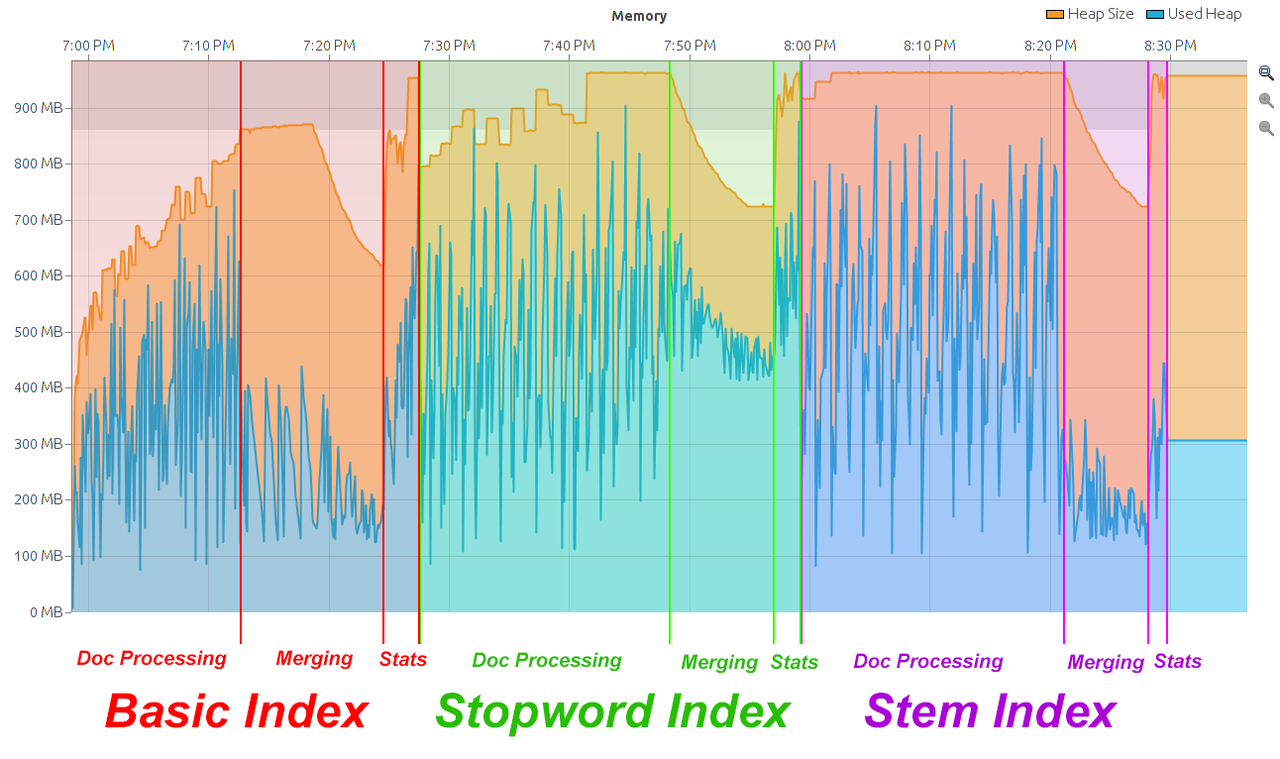
\includegraphics[width=1.8\textwidth]{profilaxis.png}
			\caption{Profiler de NetBeans para la ejecución de \textit{IndexBuilder}}
		\end{figure}
	\end{landscape}
	
	\section{Ejercicio 2: Recuperación de información.}
	%TODO
	

\end{document}